\documentclass[a4paper, 11pt]{article}
\usepackage{comment} % enables the use of multi-line comments (\ifx \fi) 
\usepackage[top = 0.5in, bottom=0.5in]{geometry}
\usepackage{color, listings, graphicx,float, booktabs, tabularx, multirow, amsmath}
\usepackage[colorlinks=true, urlcolor=blue]{hyperref}

\definecolor{codegreen}{rgb}{0,0.6,0}
\definecolor{codegray}{rgb}{0.5,0.5,0.5}
\definecolor{codepurple}{rgb}{0.58,0,0.82}
\definecolor{backcolour}{rgb}{0.95,0.95,0.92}
 
\lstdefinestyle{mystyle}{
    backgroundcolor=\color{backcolour},   
    commentstyle=\color{codegreen},
    numberstyle=\tiny\color{codegray},
    stringstyle=\color{codepurple},
    basicstyle=\footnotesize,
    breakatwhitespace=false,         
    breaklines=true,                 
    captionpos=b,                    
    keepspaces=true,                 
    numbers=left,                    
    numbersep=5pt,                  
    showspaces=false,                
    showstringspaces=false,
    showtabs=false,                  
    tabsize=2
}
\lstset{style=mystyle}

\begin{document}
\graphicspath{{./figures/}}
\noindent
\large\textbf{Kyle Salitrik (kps168)} \\
\normalsize STAT 462\\
\large{Homework 2 Report} \hfill 

%%%%%%%%%%%%%%%%%%%%%%%%%%%%%%%%%%%%%%%%%%%%%%%%%%%%%%%%%%%%%%%%%%%%
%%% SECTION: Theoretical
%%%%%%%%%%%%%%%%%%%%%%%%%%%%%%%%%%%%%%%%%%%%%%%%%%%%%%%%%%%%%%%%%%%%


\section*{Theoretical Solutions}
\subsection*{Numerical Computations}
\begin{figure}[H]
	\centering
	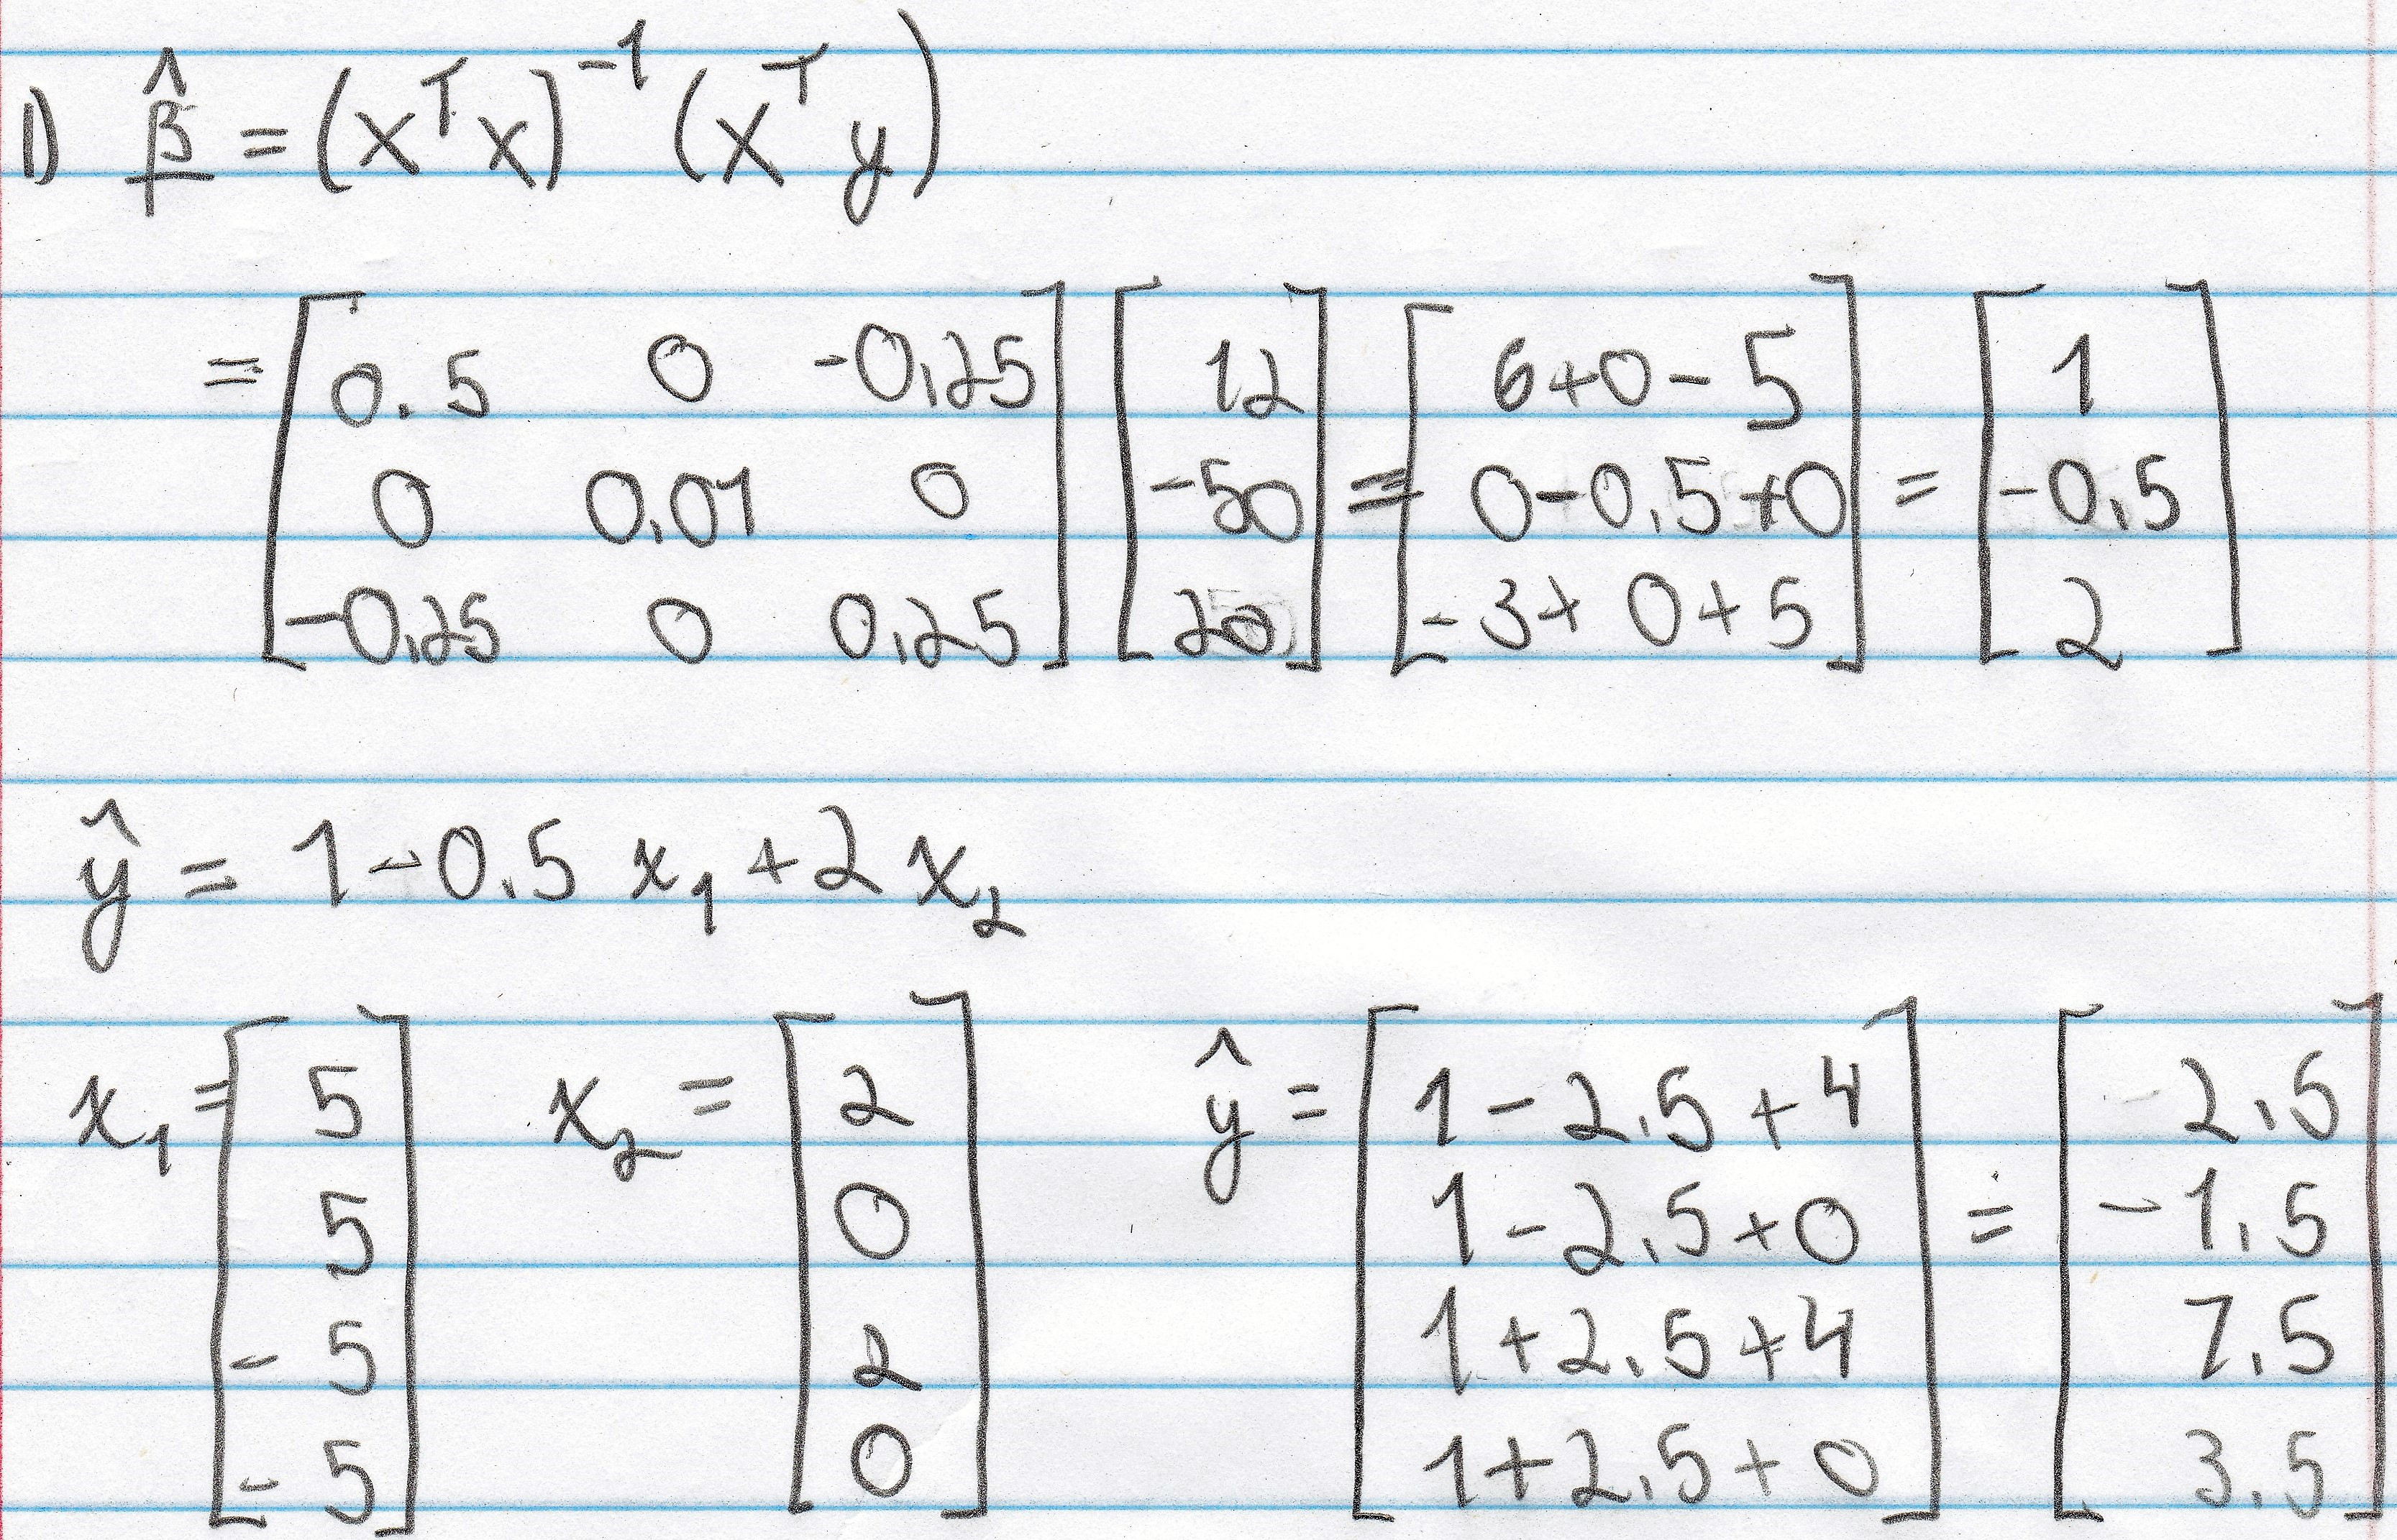
\includegraphics[width=.6\textwidth]{p1.jpg}
\end{figure}
\subsection*{Proof for $\hat{\beta_1}$}
\begin{figure}[H]
	\centering
	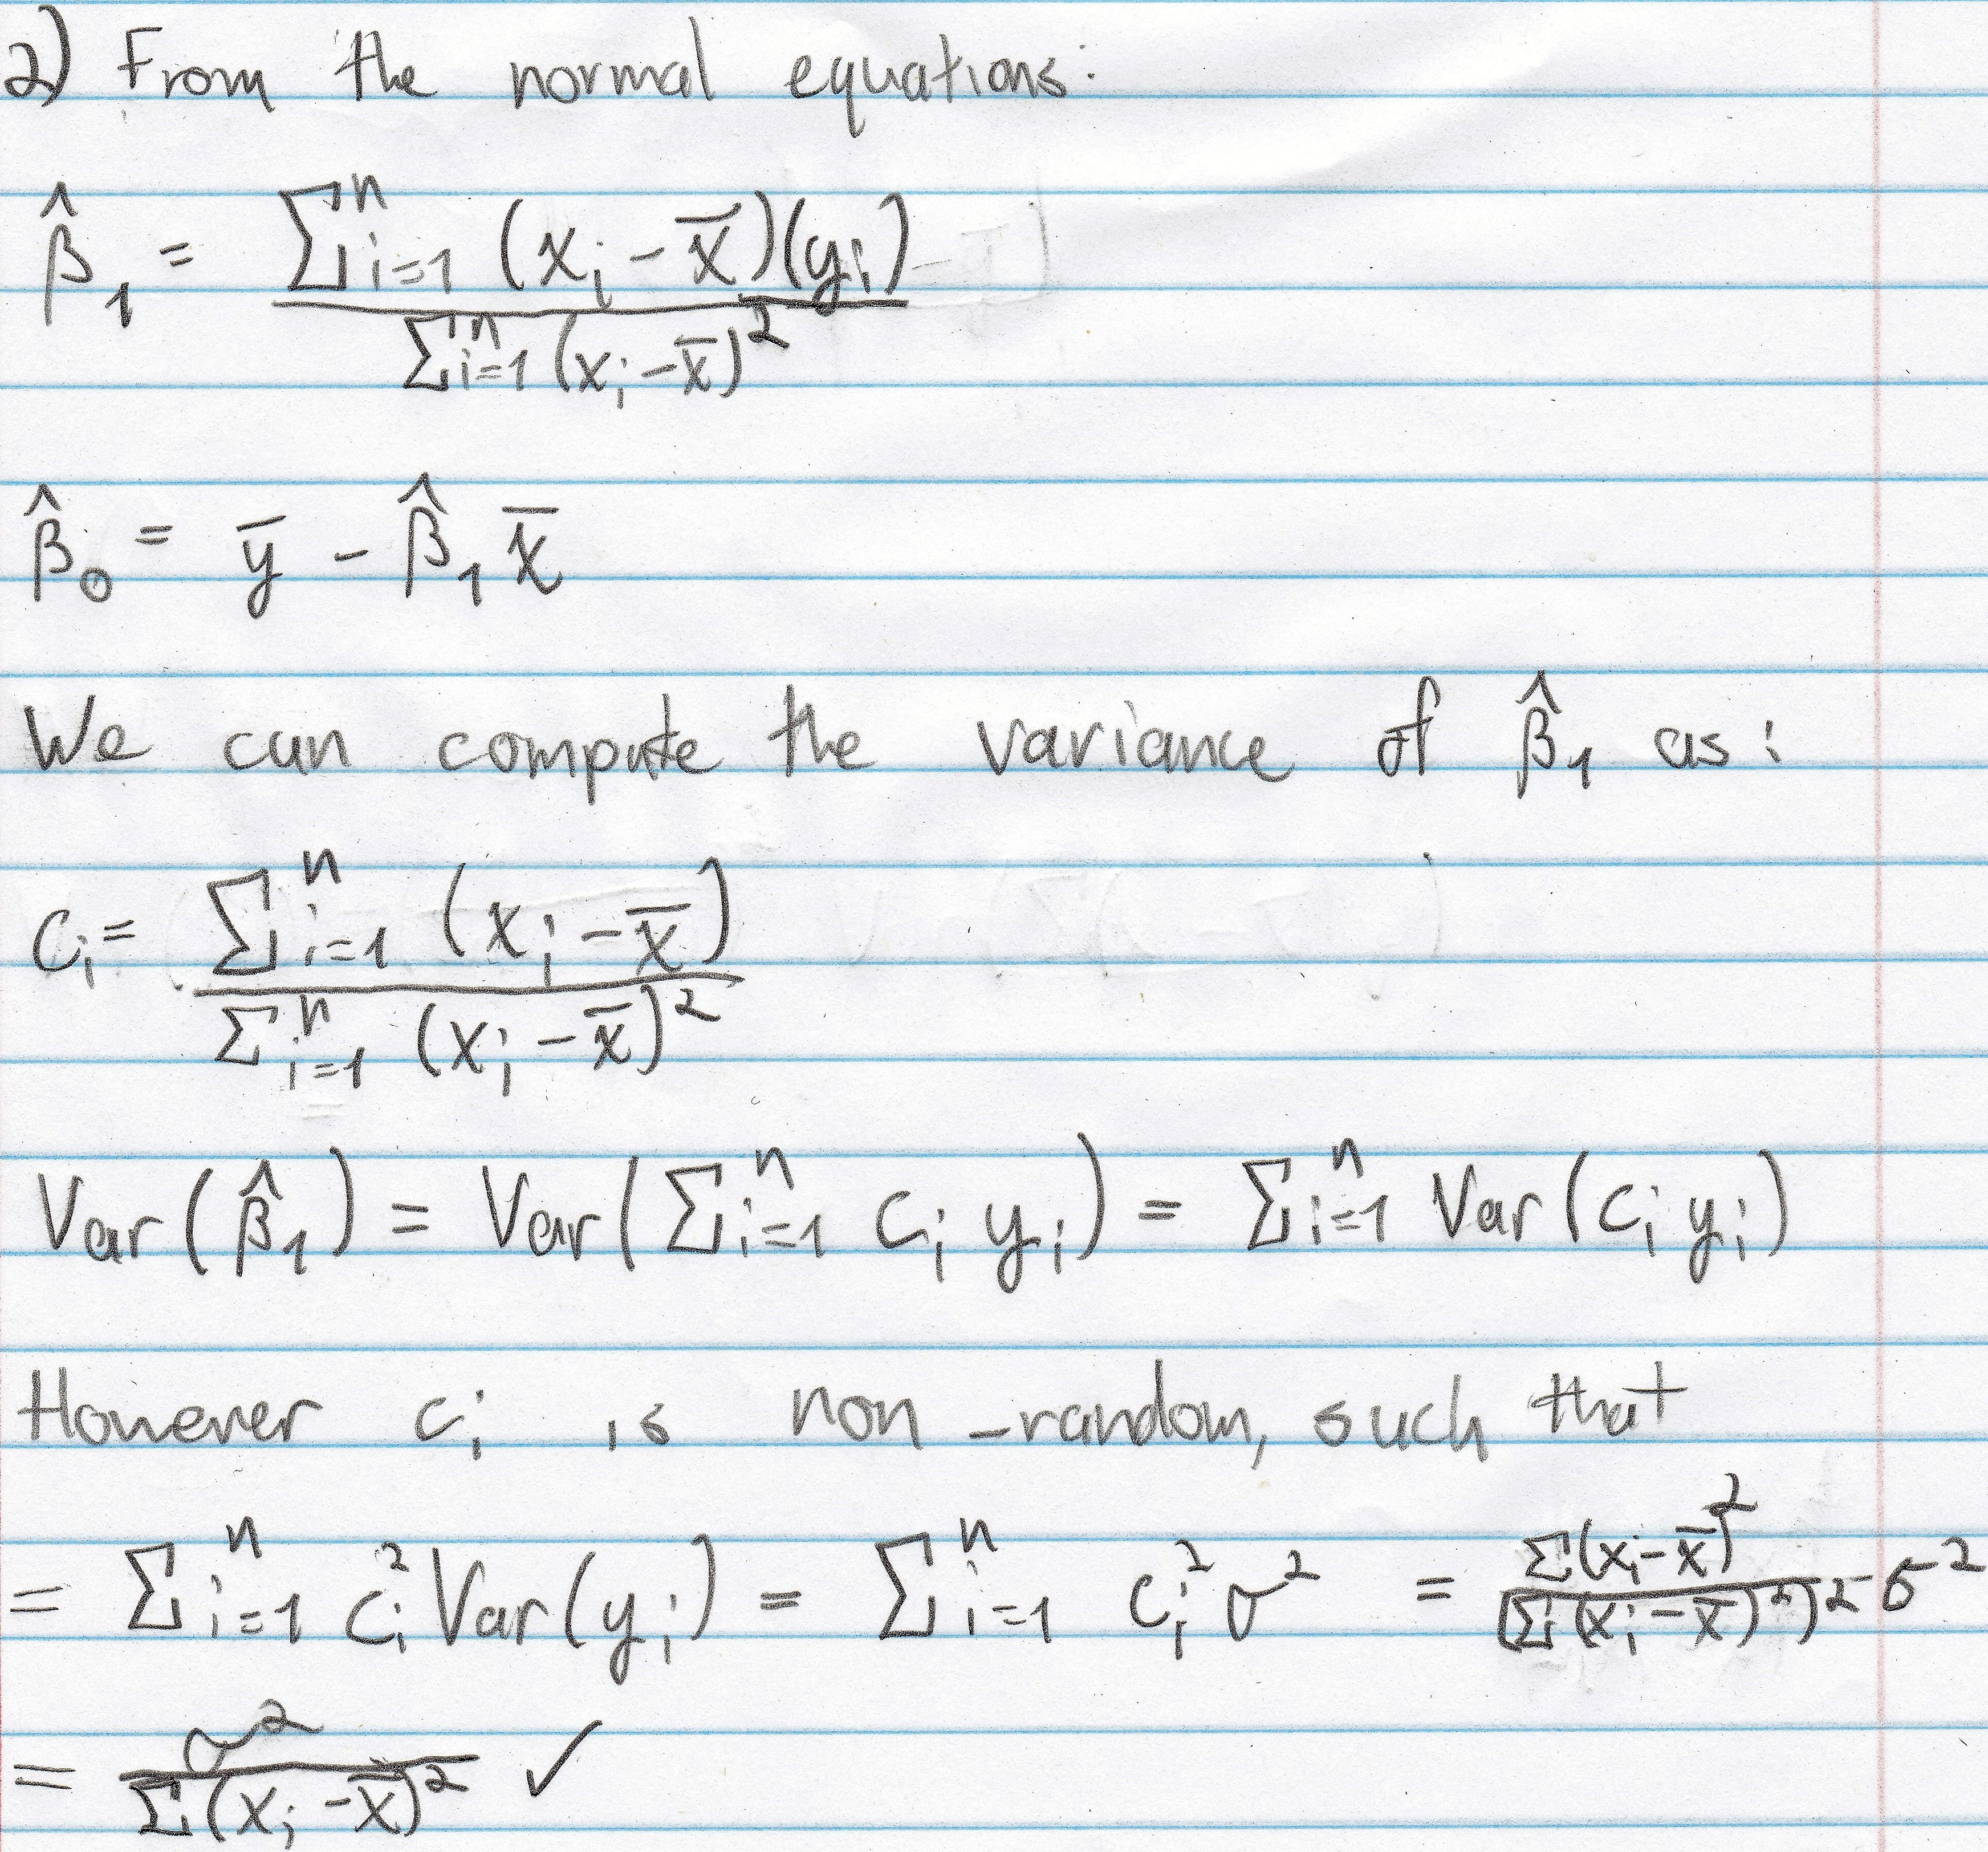
\includegraphics[width=.6\textwidth]{p2-1.jpg}
\end{figure}

\subsection*{Proof for $\hat{\beta_0}$}
\begin{figure}[H]
	\centering
	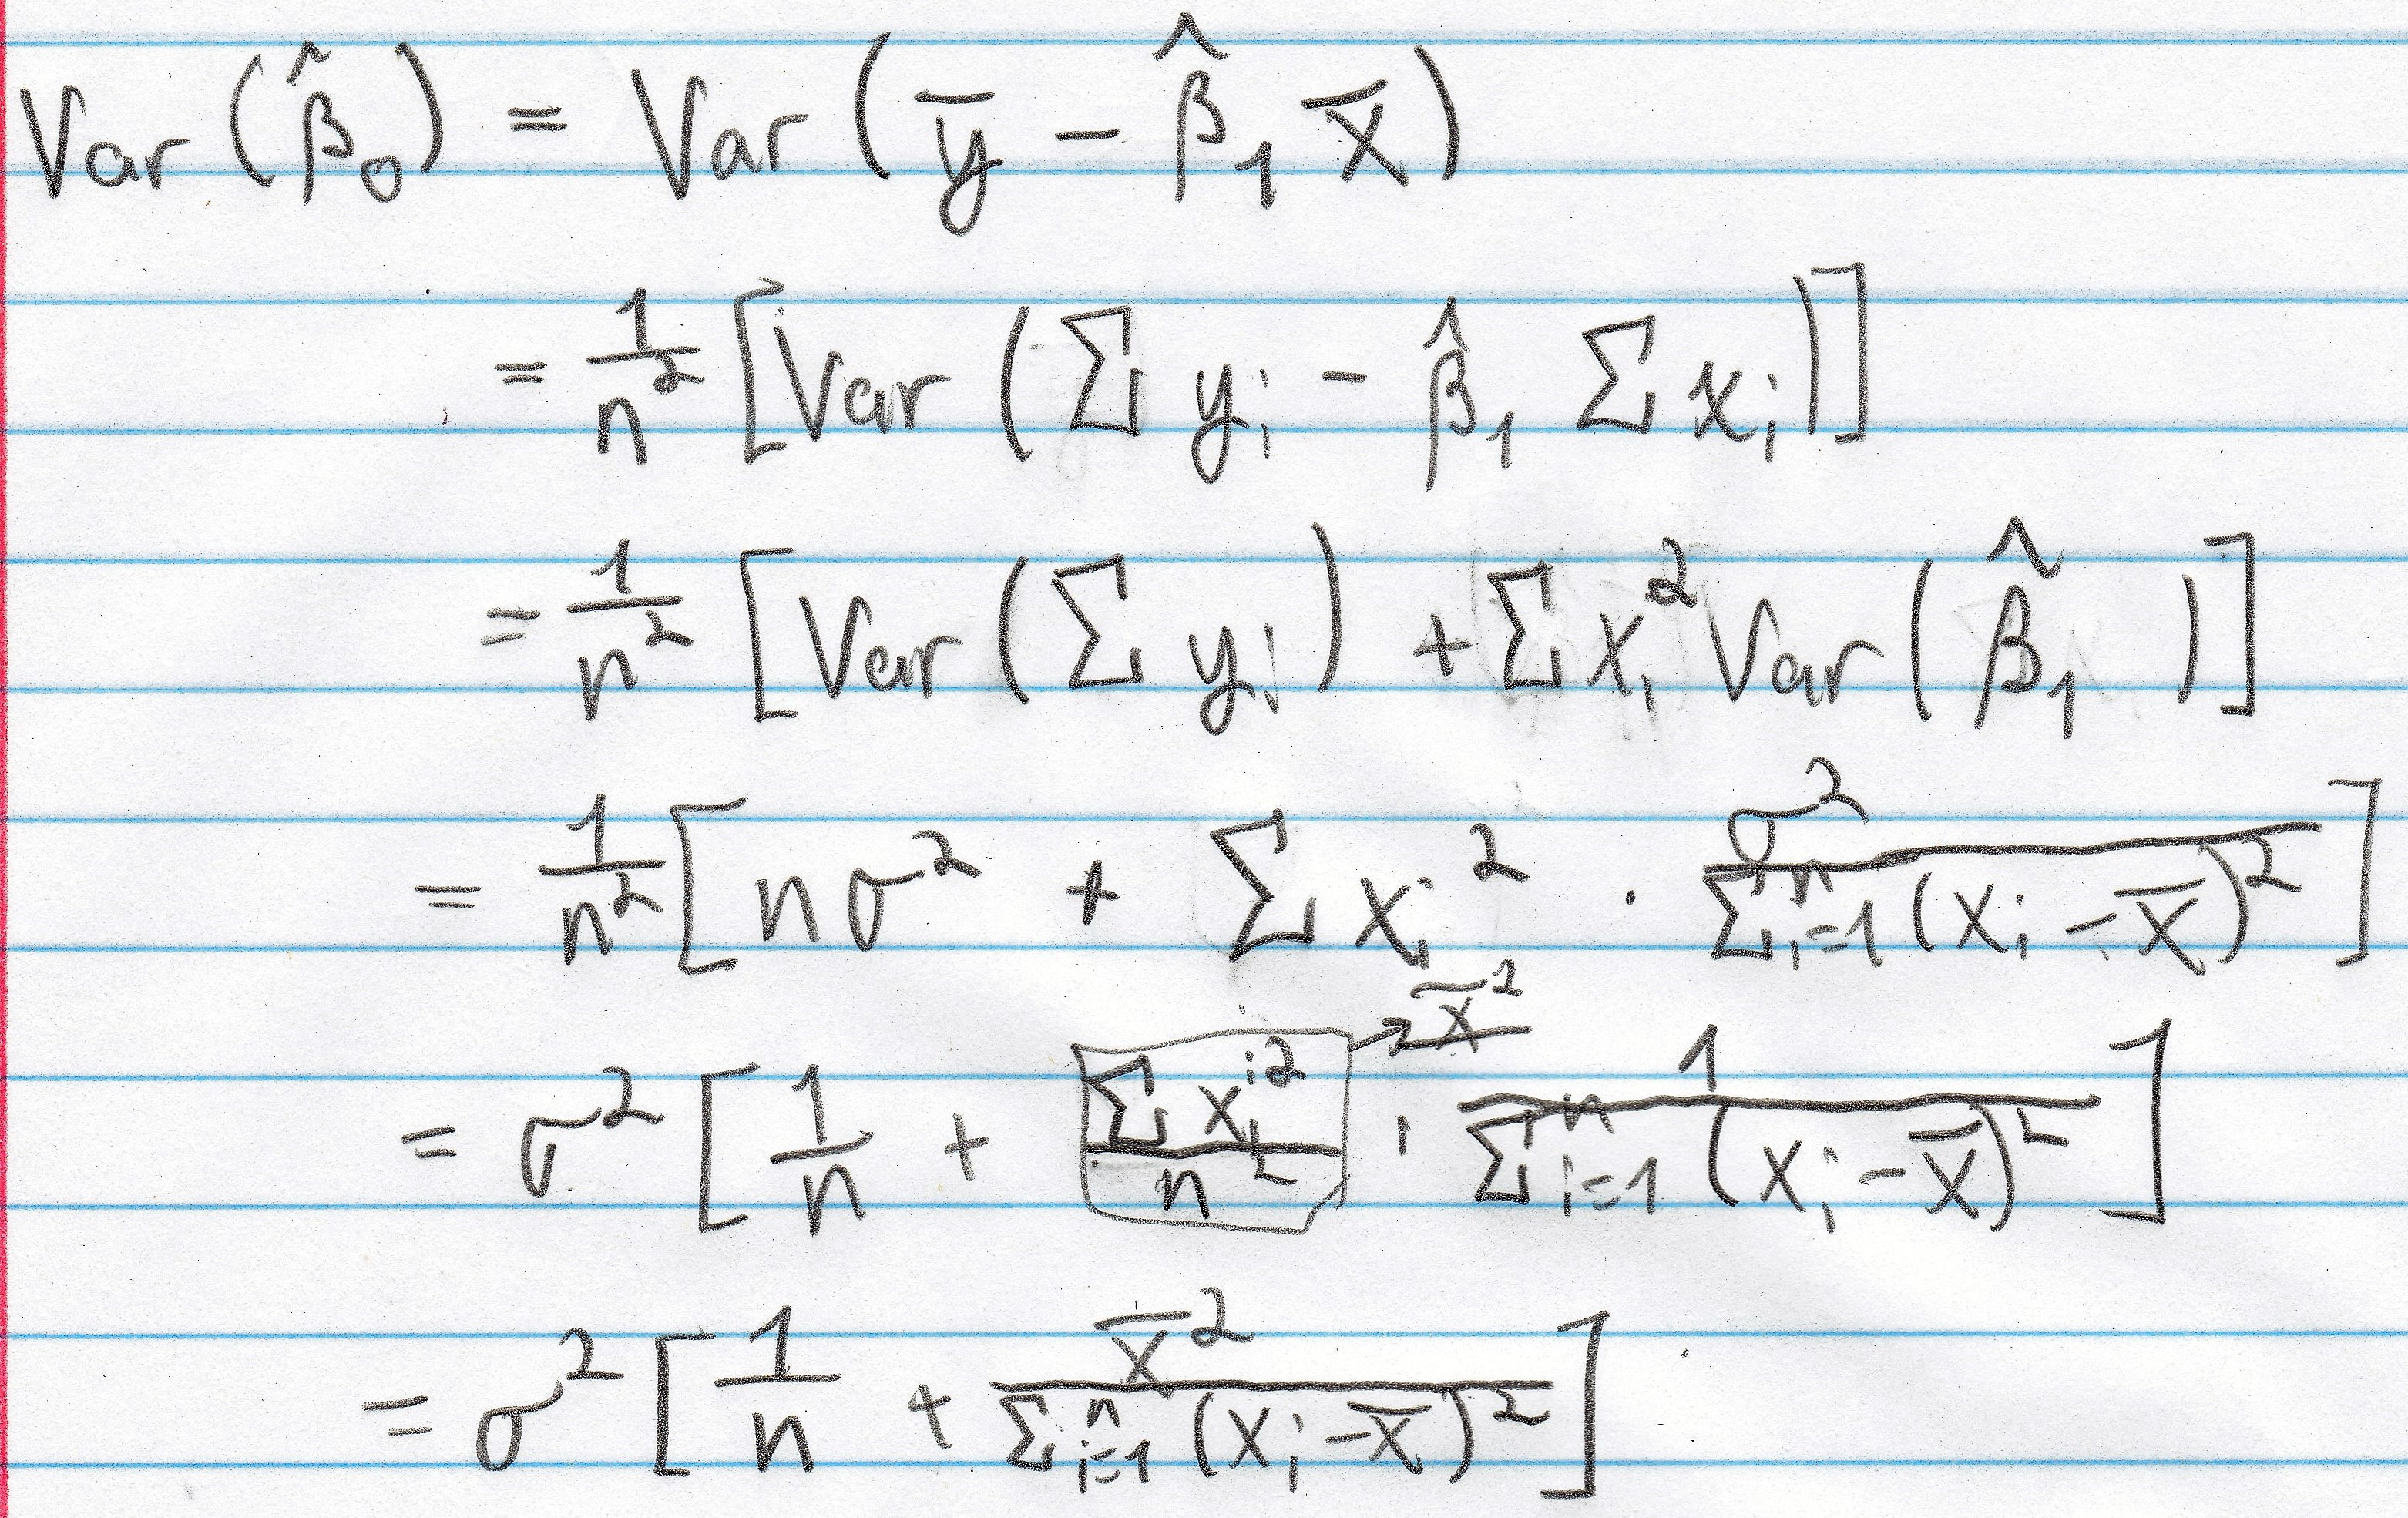
\includegraphics[width=.6\textwidth]{p2-2.jpg}
\end{figure}



%%%%%%%%%%%%%%%%%%%%%%%%%%%%%%%%%%%%%%%%%%%%%%%%%%%%%%%%%%%%%%%%%%%%
%%% SECTION: Applied
%%%%%%%%%%%%%%%%%%%%%%%%%%%%%%%%%%%%%%%%%%%%%%%%%%%%%%%%%%%%%%%%%%%%
\section*{Applied Analysis}
\subsection*{Part A}
The following reduction on the data was performed:
\begin{itemize}
	\item Samples below 2\% and above 40\% body fat were excluded. The minimum was obtained through the chart on the (\href{''https://www.acefitness.org/acefit/healthy-living-article/60/112/what-are-the-guidelines-for-percentage-of-body-fat-loss''}{\underline{ACE}}) website and maximum was set to limit outliers.
	\item The minimum height accepted was cut to be over 50 inches to remove outliers.
	\item The maximum weight was also clipped to be below 300 pounds. Although the outlier may have been legitimate, it could have also been an error.
\end{itemize}

For each individual linear model created between the response of body fat percentage and predictors weight, height and abdomen circumference, the following hypotheses were assumed.
\begin{center}
	$H_0: \beta_0 = \beta_1 = 0$\\
	$H_1: \exists \beta_i \ne 0$
\end{center}
To test these hypotheses, a T-distribution test was performed on each model with the resultant p-values:
\begin{itemize}
	\item Weight Predictor: p < 2e-16
	\item Height Predictor: p = 0.805
	\item Abdomen Circumference Predictor: p <2e-16
\end{itemize}
After performing the tests, we cannot reject the null hypothesis for the height as a predictor of body fat percentage. We can however reject the null hypotheses for the weight and abdomen circumference, implying that there is some non-zero slope relationship between the body fat percentage and these predictors.

Based on our regression models, we can obtain the following 99\% confidence intervals for $\beta_1$ of each model:
\begin{itemize}
	\item For each pound increase in weight, we are 99\% confident that, on average, the body fat percentage will increase between $~0.142$ and $~0.221$ percent.
	\item For each inch increase in height, we are 99\% confident that, on average, the body fat percentage will increase between $~0.571$ and $~0.471$ percent.
	\item For each cm increase in abdomen circumference, we are 99\% confident that, on average, the body fat percentage will increase between $~0.574$ and $~0.729$ percent.
\end{itemize}
As we can see from the confidence intervals above, not rejecting the null hypothesis for the height as a predictor is further reinforced due to the inclusion of 0 within the interval.

Looking at the coefficients of determination for each model, the values for the weight($R^2 = 0.3658$) and abdomen circumference ($R^2 = 0.6607$) models are significantly higher than that of the height model ($R^2 = 0.0611$). Again, looking at the confidence intervals, we can see that the abdomen circumference has a lower bound that is much higher (more than twice) than the upper bound for the weight, indicating that abdomen circumference is the strongest predictor out of the three.

\subsection*{Part B}
Next, we are interested whether or not there is evidence to indicate that the average increase in body fat percentage for each cm increase of abdomen circumference is actually greater than $0.5\%$. A t-test was performed on the following hypotheses.
\begin{center}
	$H_0: \beta_1 \leq 0.5$\\
	$H_1: \beta_1 > 0.5$
\end{center}

The t-value obtained was $5.067856$ and an underlying normal distribution was assumed for $\beta_1$. As such, the p-value was calculated using $1-pnorm(t)$ in R to obtain a p-value of $2.011611*10^-7$. With the p-value confirming that our confidence interval for the slope is correct, and that the actual value for $\beta_1$ is over $0.5$.

\subsection*{Part C}
The following figure includes the residuals from the abdomen circumference predictor model plotted against weight, height, neck circumference, chest circumference, hip circumference, thigh circumference, knee circumference, ankle circumference, biceps circumference, forearm circumference, and wrist circumference.
\begin{figure}[H]
	\centering
	%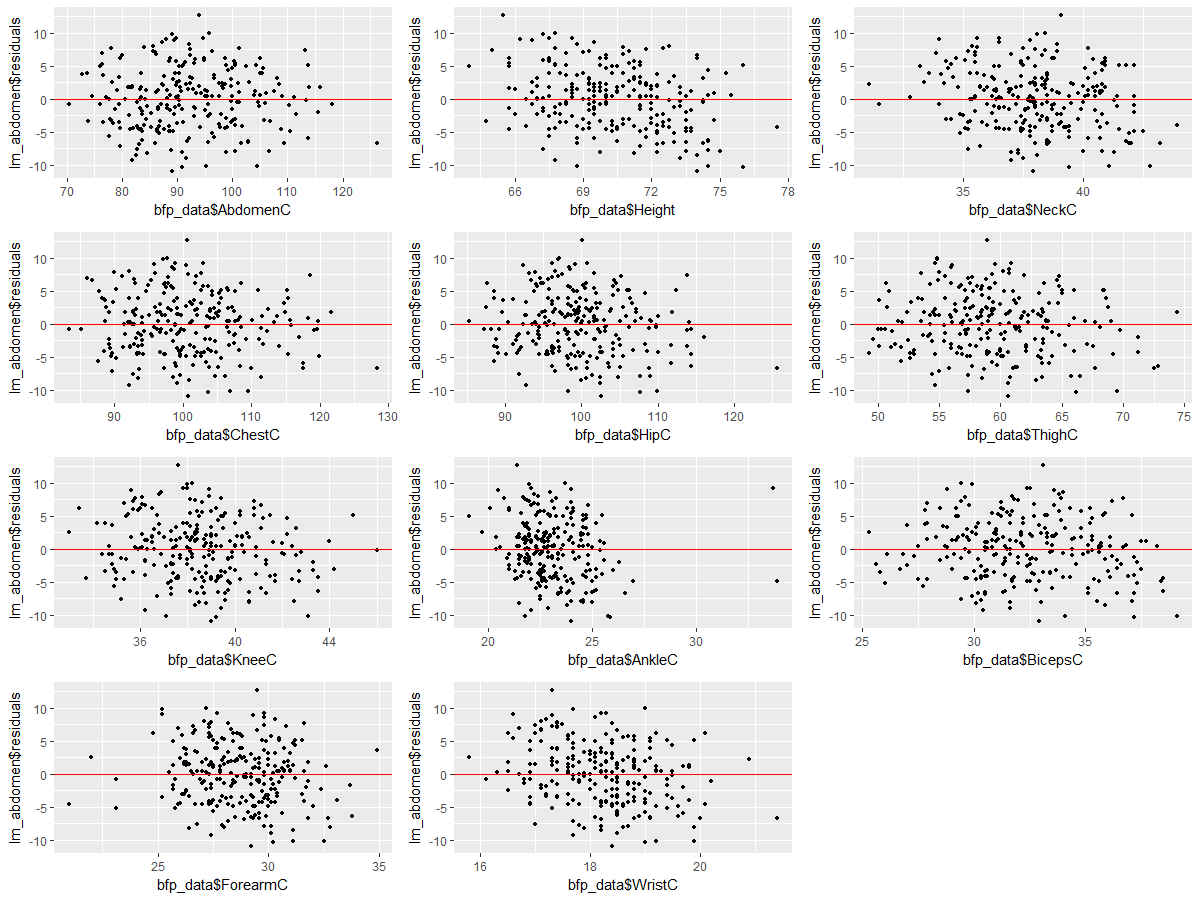
\includegraphics[width=8in, angle=90, origin=c]{plots.png}
	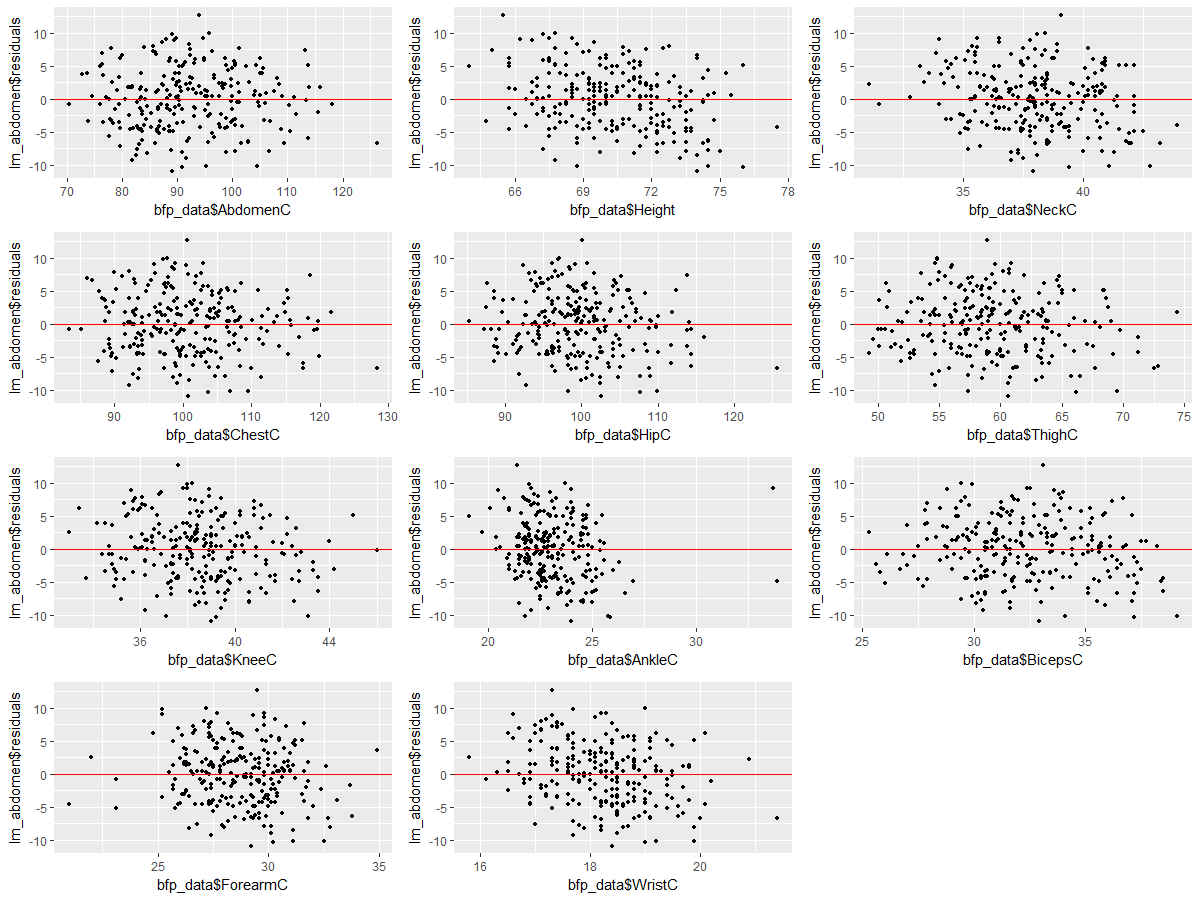
\includegraphics[width=\textwidth]{plots.png}
\end{figure}

From these plots, we can see that there may potentially be a relationship between the body fat percentage and the ankle circumference. It may make sense that wrist circumference could  indicate an increase in fat percentage, based on where the wrist is defined to lie. If the measurements were taken further up the forearm where one would wear a watch, as opposed to the actual wrist joint, then the measurement may indicate something about the body fat percentage.

\subsection*{Part D}
Next if we fit a linear model (stated below) using all of these variables to predict the body fat percentage, we will be able to compare it to the reduced (abdomen circumference) only model in order to determine whether the other predictors are actually necessary. The test statistic used for this was an f-distribution (also noted below).
\begin{align*}
 BFP = & \beta_0 + \beta_1*AbdomenC + \beta_2*Weight + \beta_3*Height + \beta_4*NeckC + \\ 
 & \beta_5*ChestC + \beta_6*HipC + \beta_7*ThighC + \beta_8*KneeC + \beta_9*AnkleC + \\ 
 &\beta_10*BicepsC + \beta_11*ForearmC + \beta_12*WristC + \epsilon\\
  \widehat{BFP} = & 1.36987591 + 0.98199026*AbdomenC - 0.04420200*Weight - \\
  &0.26163775*Height - 0.38320373*NeckC - 0.10481085*ChestC - \\
  & 0.20730987*HipC + 0.06182966*ThighC + 0.14670469*KneeC + \\
  &0.12543748*AnkleC + 0.17961142*BicepsC + 0.23096461*ForearmC - \\ 
  &1.40026669*WristC\\
\hat{\sigma}^2=& 17.9776\\
R^2 = &0.7304
\end{align*}

The F-value used in the f-test was computed to be the following value, and using the given parameters:

\begin{align*}
	 H_0:\quad &\omega: y_i = \beta_0 + \beta_1 * AbdomenC_i \\
	 H_1:\quad &\Omega: \text{The full model stated above where } \exists \beta_i \ne 0, i = [2, 12]\\
	 n = &246, \quad p = 13, \quad q = 2 \\
	 F \sim& F_{11, 233}\\
	 F_{value} = &5.482263\\
	 p-value = &9.011923*10^{-8}
\end{align*}

Based on the results of the F-test and looking at the R-squared values, we cannot reject the  null hypothesis that the abdomen circumference model is not strong enough to predict the body fat percentage accurately.

%%%%%%%%%%%%%%%%%%%%%%%%%%%%%%%%%%%%%%%%%%%%%%%%%%%%%%%%%%%%%%%%%%%%
%%% SECTION: CODE APPENDIX
%%%%%%%%%%%%%%%%%%%%%%%%%%%%%%%%%%%%%%%%%%%%%%%%%%%%%%%%%%%%%%%%%%%%

%\newpage
\section*{R Output}
This section contains the output from the R console for important values and summaries.
\lstinputlisting[language=R]{./code/output.txt}

\end{document}